% Seccion de Diseno y construccion 

%%\chapter{Integración de componentes}
\label{chapter:diseno}
\section{Diseño y Construcción}

Con el objetivo de construir un robot humanoide que lograra buscar y patear una pelota, el primer paso debi\'o ser la construcci\'on del robot en si para tal fin se procedió a la elección del diseño y al armado de piezas. En la siguiente sección se presenta las distintas partes utilizadas tanto en componentes de software y hardware como la integración física de los componentes.

\subsection{Componentes de hardware}
Para armar el robot es necesario tener claro los distintos componentes de hardware que se tienen disponibles y que se necesitan por ello se presenta a continuacion una descripción de todos los elementos utilizados. 

\begin{itemize}
\item Bioloid Premium kit: Es un kit (figura ~\ref{fig:kit}) de robótica con piezas modulares que permite armar diferentes tipos de robot pero principalmente humanoides. El fabricante, ROBOTIS, incluye un manual con varios modelos de robots con instrucciones de ensamblaje. Provee una tarjeta controladora, CM-510, a la que se conectan los motores Dynamixel y algunos sensores que se programan a través de la interfaz de ‘RoboPlus’. \cite{robotics}

\end{itemize}

\begin{figure}[hbtp]

\centering
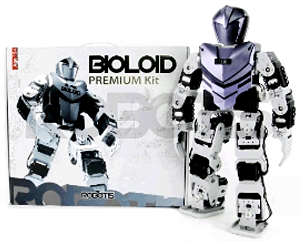
\includegraphics[scale=0.5]{imagenes/product_bioloid17.png}
\caption{Bioloid Premium Kit}
\label{fig:kit}
\end{figure}

\begin{itemize}

\item Motores Dynamixel Ax-12+: Son actuadores inteligentes y modulares que incorporan un reductor de engranajes, un motor DC  (figura ~\ref{fig:motoresDc}) de presión y un circuito de control con funcionalidad de red lo cual permite formar series de motores, todo en un solo paquete \cite{manual}. 
\end{itemize}

\begin{figure}[hbtp]

\centering
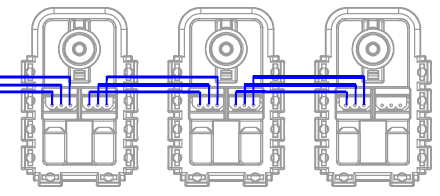
\includegraphics[scale=0.5]{imagenes/AX-12_serie.png}
\caption{Motores Dynamixel conectados en serie}
\label{fig:motoresDc}
\end{figure}

\begin{itemize}
\item Gyro: Es un giroscopio (figura ~\ref{fig:gyro}) de la marca Robotis que mide la velocidad angular, diseñado para mantener el balance del robot y ser usado para otras aplicaciones de movimiento. \cite{gyro} 

\end{itemize}

\begin{figure}[hbtp]
\centering

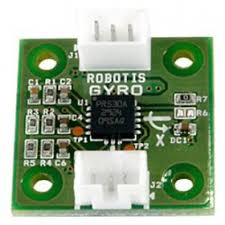
\includegraphics[scale=0.3]{imagenes/gyro.jpg}

\caption{Sensor Gyro}
\label{fig:gyro}
\end{figure}

\begin{itemize}
\item Arbotix: El controlador ArbotiX es una solución de control avanzado para manejar servos Dynamixel AX/MX/RX/EX y robots
basados en Bioloid. Incorpora un potente microcontrolador AVR, radio inalámbrica XBEE, conductores de motor dual, y cabeceras
de estilo servo de 3 pines para E/S digital y analógica.\cite{arbotix}

\end{itemize}

%\begin{figure}[hbtp]
%\centering
%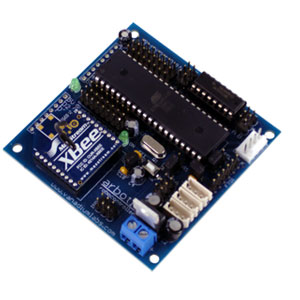
\includegraphics[scale=0.5]{imagenes/ARBOTIX.JPG}
%\caption{Tarjeta controladora ArbotiX}
%\end{figure}

\begin{itemize}
\item FTDI (Future Technology Devices International) : Es una tarjeta controladora  (figura ~\ref{fig:ftdi}) que ofrece el servicio de conversión de  datos de USB a UART. Permite la comunicación entre diferentes dispositivos \cite{ftdi}.

\end{itemize}

\begin{figure}[hbtp]
\centering

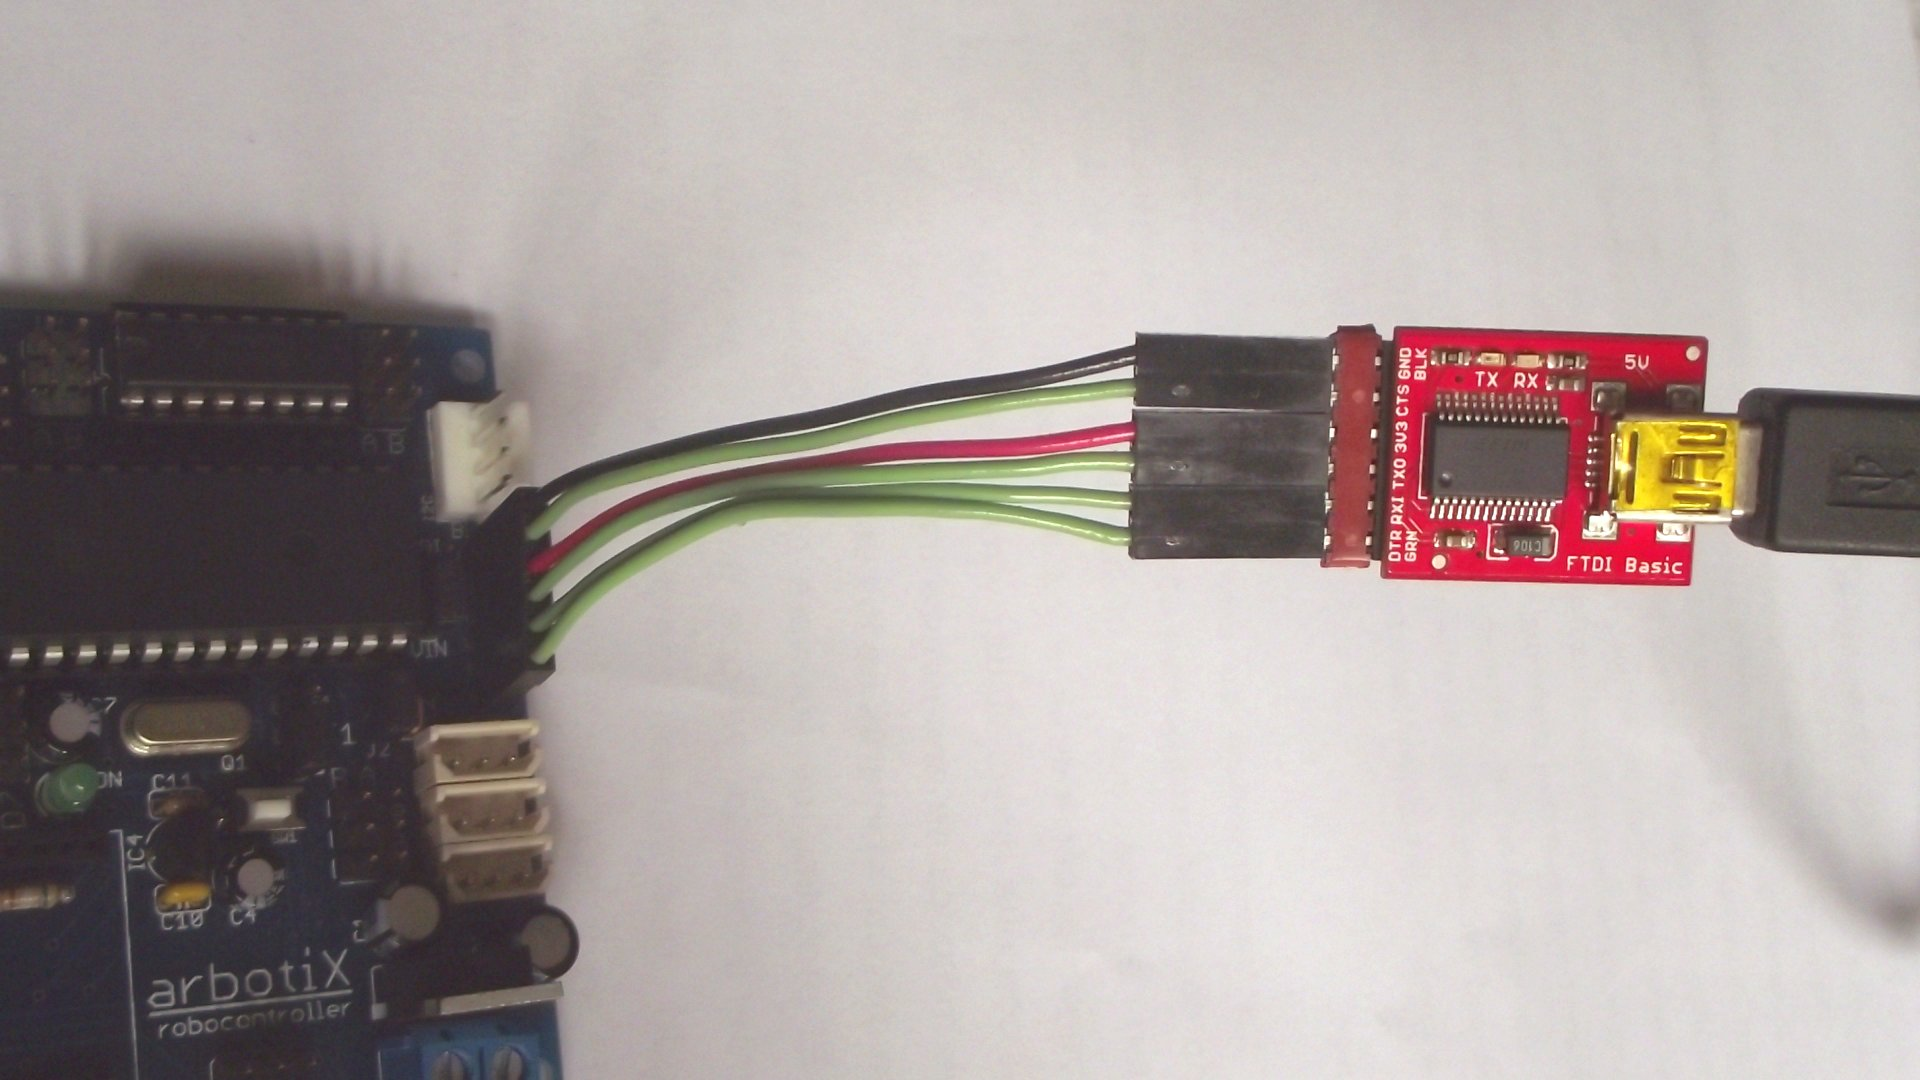
\includegraphics[scale=0.06]{imagenes/DSCF1162.jpg}

\caption{Chip FTDI conectado a la tarjeta Arbotix}
\label{fig:ftdi}
\end{figure}

\begin{itemize}
\item Extensor de puertos bioloid : Permite aumentar el número de cadenas de servos conectados a la tarjeta. (figura ~\ref{fig:ext}) \cite{hub} 
\end{itemize}

\begin{figure}[hbtp]
\centering
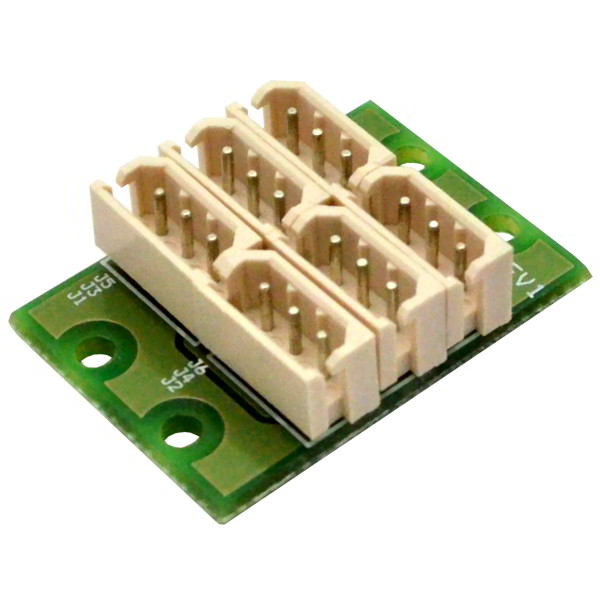
\includegraphics[scale=0.1]{imagenes/Dynamixel-AX-MX-6-Port-Extension-Hub-600x600.jpg}


\caption{Extensor de puertos bioloid}
\label{fig:ext}
\end{figure}

\begin{itemize}
\item Servo motor anal\'ogico micro TG9 e: Es un pequeño servomotor  (figura ~\ref{fig:Servo}) cuyo torque alcanza 1.50 kg-cm y una velocidad de 60 por segundo. Permite ser controlado en posición en un rango de 180. \cite{microservo}  

\end{itemize}

\begin{figure}[hbtp]
\centering
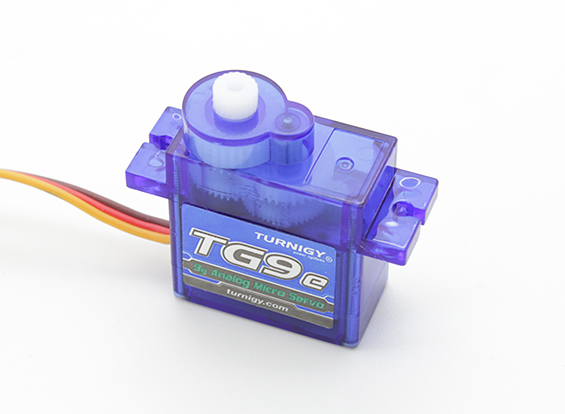
\includegraphics[scale=0.1]{imagenes/turnigy.jpg}

\caption{Servo motor analógico}

\label{fig:Servo}
\end{figure}

\begin{itemize}
\item Raspberry Pi: La Raspberry Pi (figura ~\ref{fig:Raspe}) es un ordenador del tamaño de una tarjeta de crédito a la que se puede conectar un televisor y un teclado. Se trata de un pequeño ordenador capaz de ser utilizado en proyectos de electrónica y para muchas de las tareas que una PC de escritorio hace, como hojas de cálculo, procesadores de texto y juegos \cite{raspberry}. 

\end{itemize}

%imagen tomada de: %http://rayhightower.com/blog/2012/12/03/ruby-on-raspberry-pi/
\begin{figure}[hbtp]
\centering

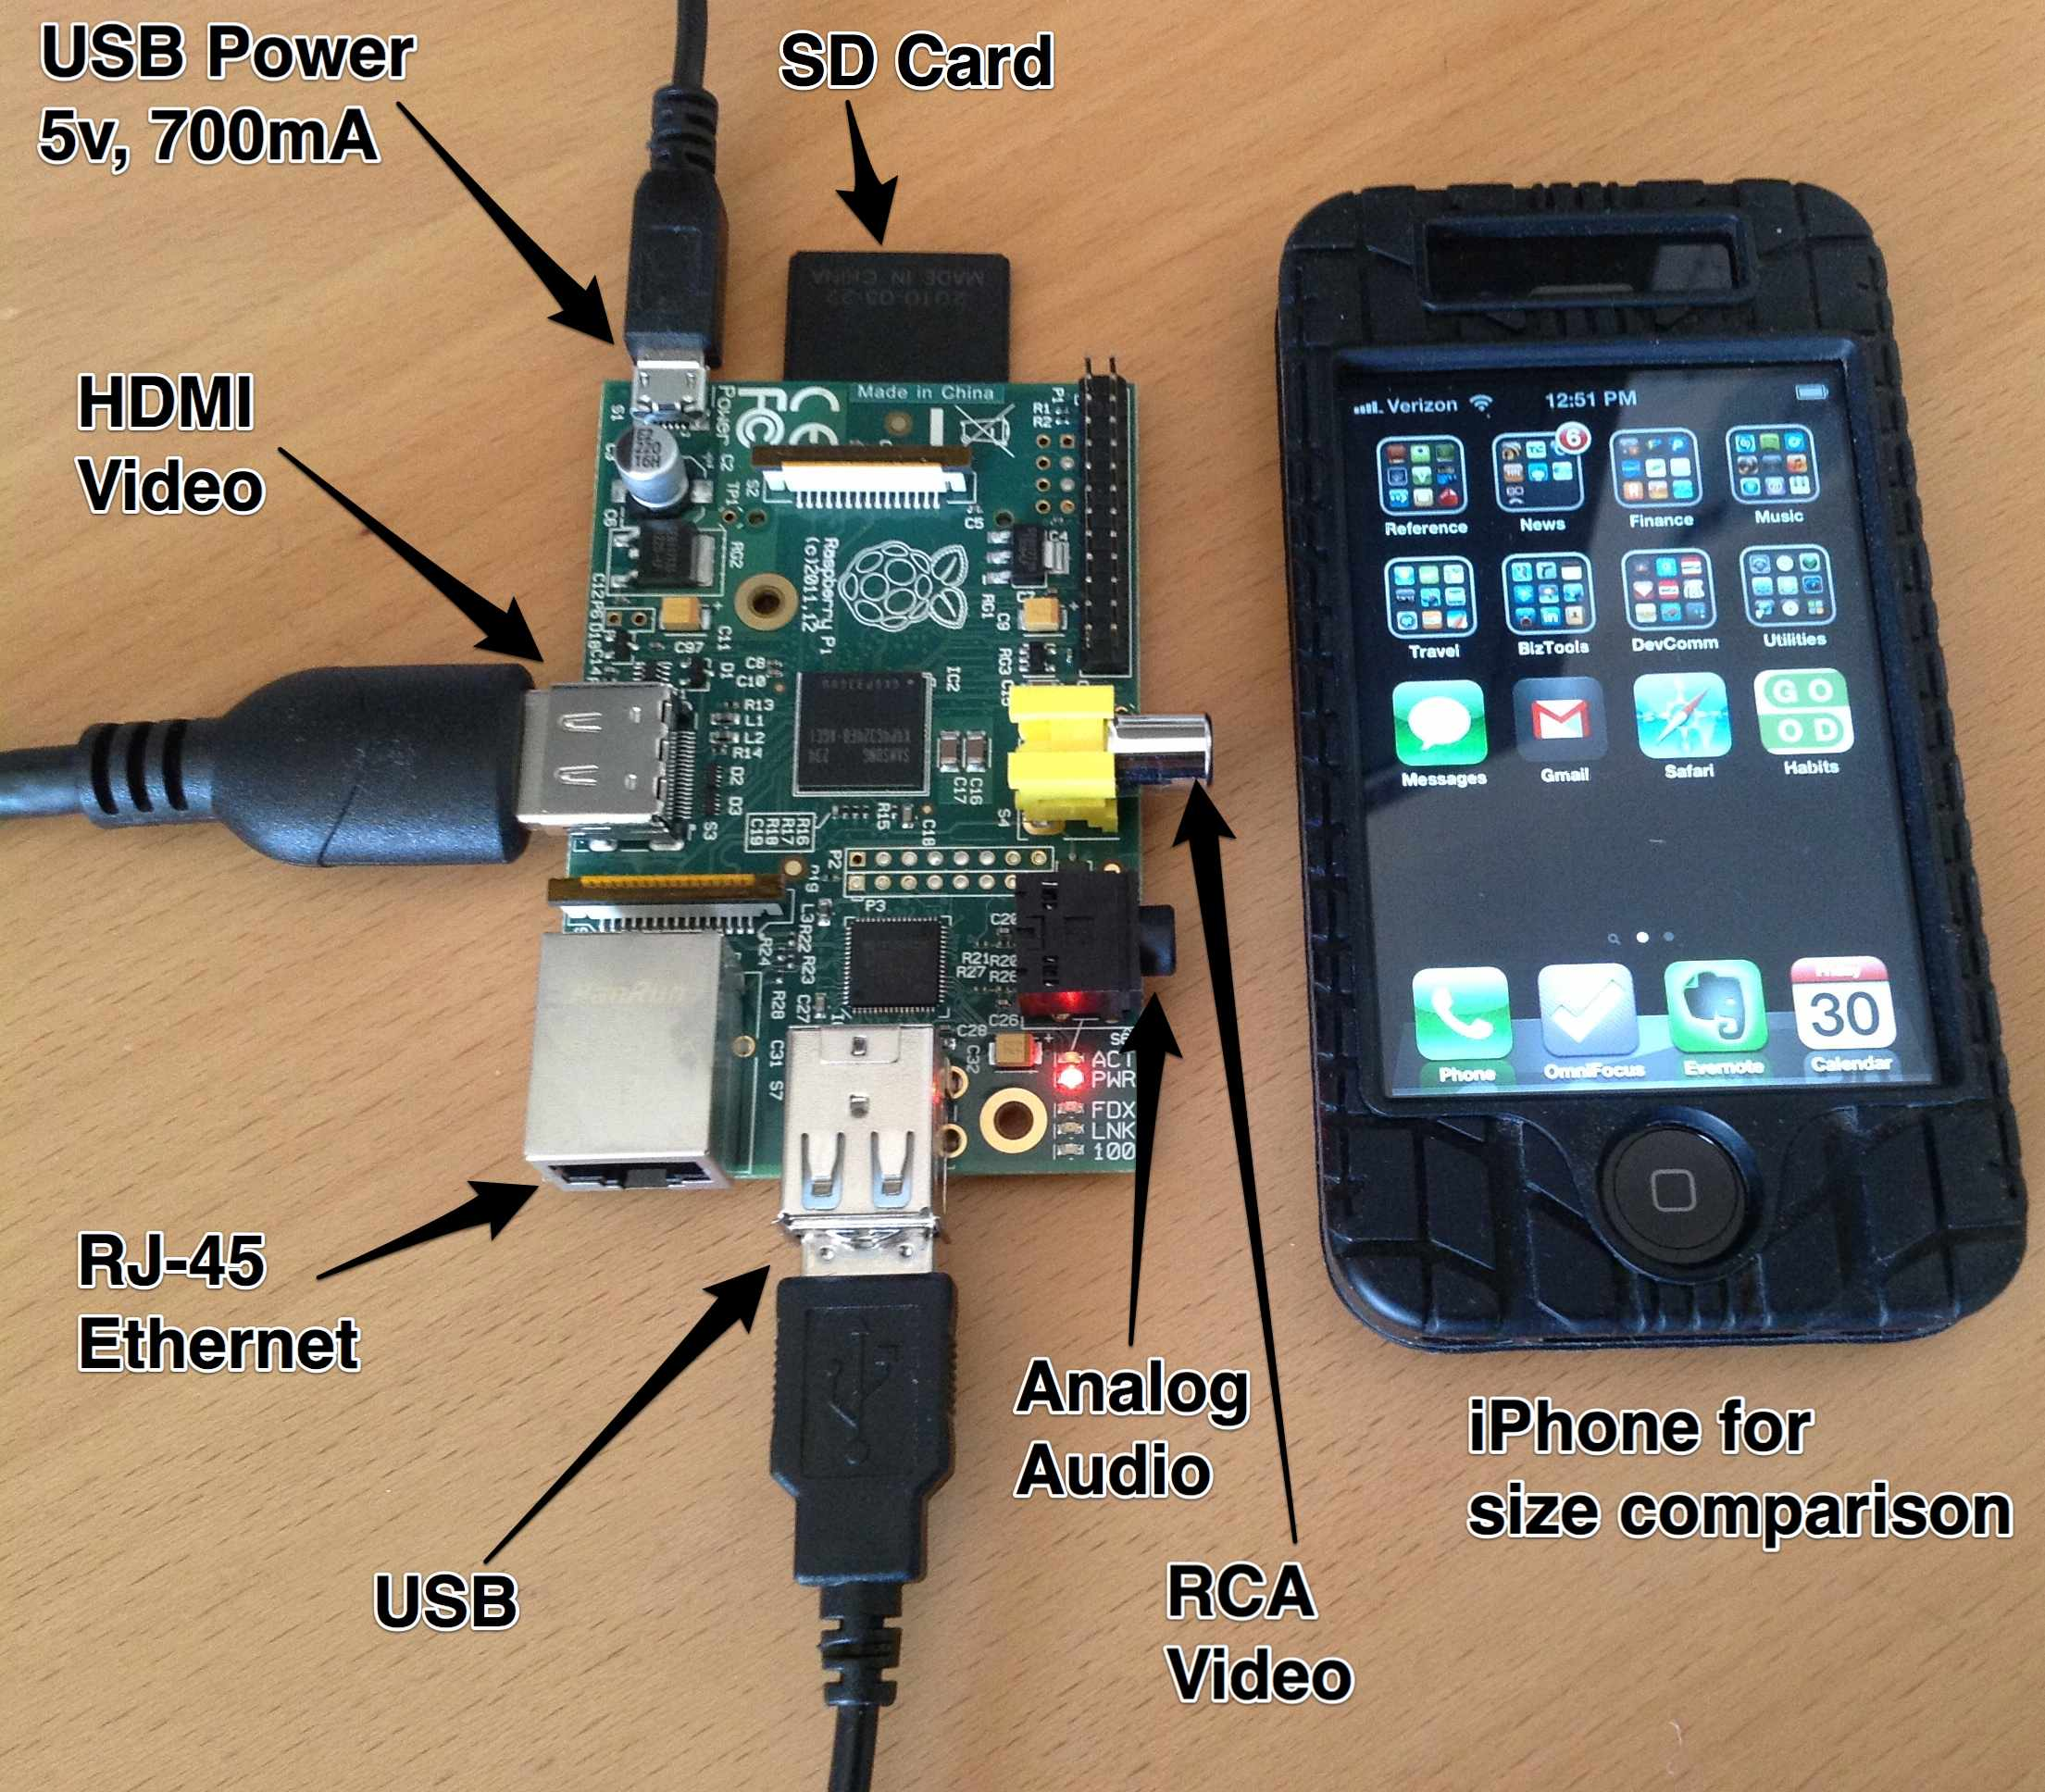
\includegraphics[scale=0.1]{imagenes/raspberry_pi_iphone.jpg}
\caption{Tarjeta Raspberry Pi con descripción de los puertos}
\label{fig:Raspe}
\end{figure}

\begin{itemize}
\item C\'amara Raspberry Pi: Es un sensor encargado de captar imagenes y grabar videos de alta definicion. Se conecta a la Raspberry Pi con un cable de cinta plana de 15 cm en el puerto CSI. Tiene 5 megapíxeles de foco fijo que soporta los modos de vídeo de 1080x30, 720x60 y VGA90. Puede ser manejada con las librerías MMAL, V4L u otras librerías de terceros como la de Python.(figura ~\ref{fig:came}) \cite{raspberrycam} %(http://www.raspberrypi.org/products/camera-module/)

\end{itemize}

\begin{figure}[hbtp]
\centering
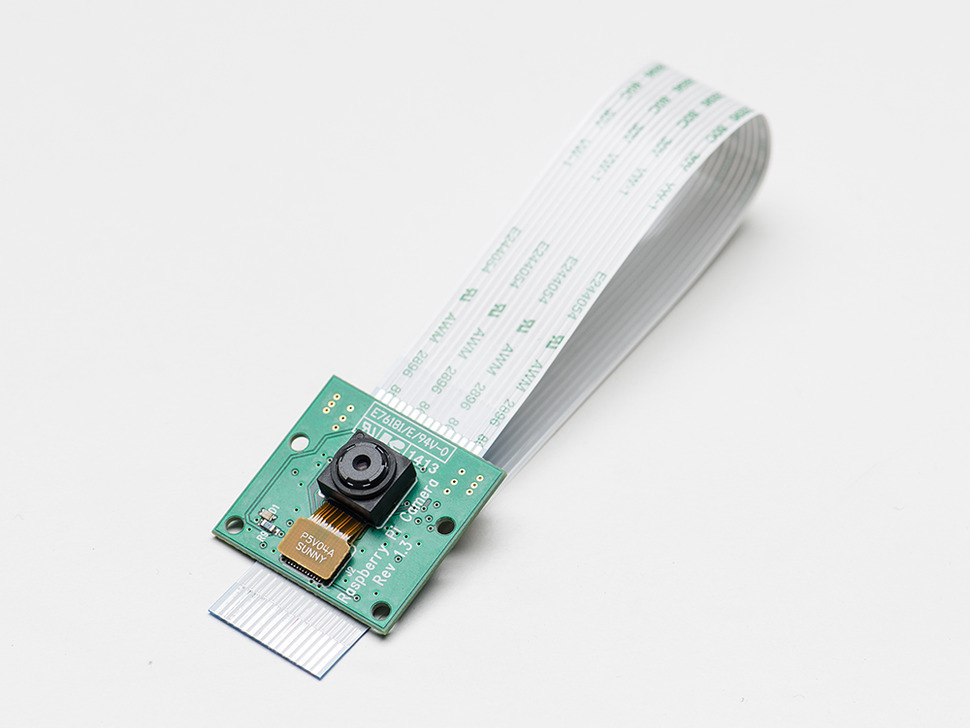
\includegraphics[scale=0.3]{imagenes/1367-01.jpg}


\caption{C\'amara Raspberry Pi}
\label{fig:came}
\end{figure}


\begin{itemize}
\item Batería de polímero de litio (Lipo): Es la fuente de poder usada para los motores y componentes electr\'onicos. La batería usada es de 11.1 voltios y 1 amperio. \cite{bateria}
\end{itemize}


\begin{figure}[hbtp]
\centering
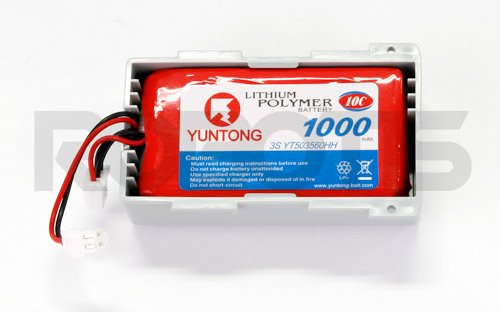
\includegraphics[scale=0.3]{imagenes/R-LIPOBAT.jpg}
\caption{Batería Lipo}
\label{bateria}
\end{figure}

\begin{itemize}
\item Circuito con regulador de 5v: Es un circuito diseñado y construido para este proyecto cuya finalidad es regular la entrada de la corriente. Por una de las salidas se expulsa 5v y por la otra se mantiene el mismo voltaje de entrada. 
\end{itemize}



%\begin{figure}[hbtp]
%\centering
%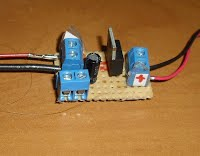
\includegraphics[scale=0.7]{imagenes/circuito.jpg}
%\caption{Lipo}
%\end{figure}


\subsection{Herramientas software }

Para la programación del robot se necesitaron distintas herramientas de software que permitieron ir desarrollando el comportamiento del robot. A continuación se presenta la descripción de las herramientas utilizadas. 

\begin{itemize}
\item Pypose: Software especializado en el control de los servomotores Dynamixel Ax-12. Una de las más importantes características es que, luego de haber fijado a mano las posiciones de los motores, permite la lectura simultánea de esas posiciones para captar la pose del robot. Con esta herramienta es posible formar una secuencia de poses que generen un movimiento, por ejemplo, caminar. \cite{pypose}

\item ROS: ROS (Robot Operating System) es un framework que proporciona bibliotecas y herramientas para ayudar a los desarrolladores de software a crear aplicaciones robóticas. Proporciona abstracción de hardware,  de dispositivos, bibliotecas, visualizadores, paso de mensajes, gestión de paquetes y más. ROS se encuentra bajo licencia de código abierto, la licencia BSD.

\item OpenCv (Open Source Computer Vision Library): Es una librería de visión de computadoras y aprendizaje de máquinas de código abierto. Ha sido diseñada para acelerar el uso de la percepción de m\'aquinas y para proveer una estructura común en las aplicaciones de visión de computadoras. Registrada bajo la licencia BSD, de código abierto. \cite{opencv}

\item IDE Arduino: Es un entorno de desarrollo para escribir y cargar código en la tarjeta Arduino. Otras tarjetas con microcontroladores AVR también son compatibles, como la ArbotiX. El lenguaje de programación del IDE de Arduino es una implementación de Wiring el cual esta basado en Processing.  \cite{arduino}

\end{itemize}

\subsection{Construcción}
Para la construcción del robot se utilizó el kit de piezas Bioloid Premium de marca Robotis el cual incluye motores Dynamixel Ax-12+, una tarjeta controladora CM-510, un sensor Gyro, un manual, entre otros elementos. El manual incluye las instrucciones de como armar varios modelos de humanoide, el utilizado en este proyecto es el tipo B, haciendo uso de 16 motores. En la figura ~\ref{fig:frontal} y ~\ref{fig:trasera1} se puede observar la estructura del robot que aparece en el manual del kit. 

\begin{figure}[hbtp]
\centering
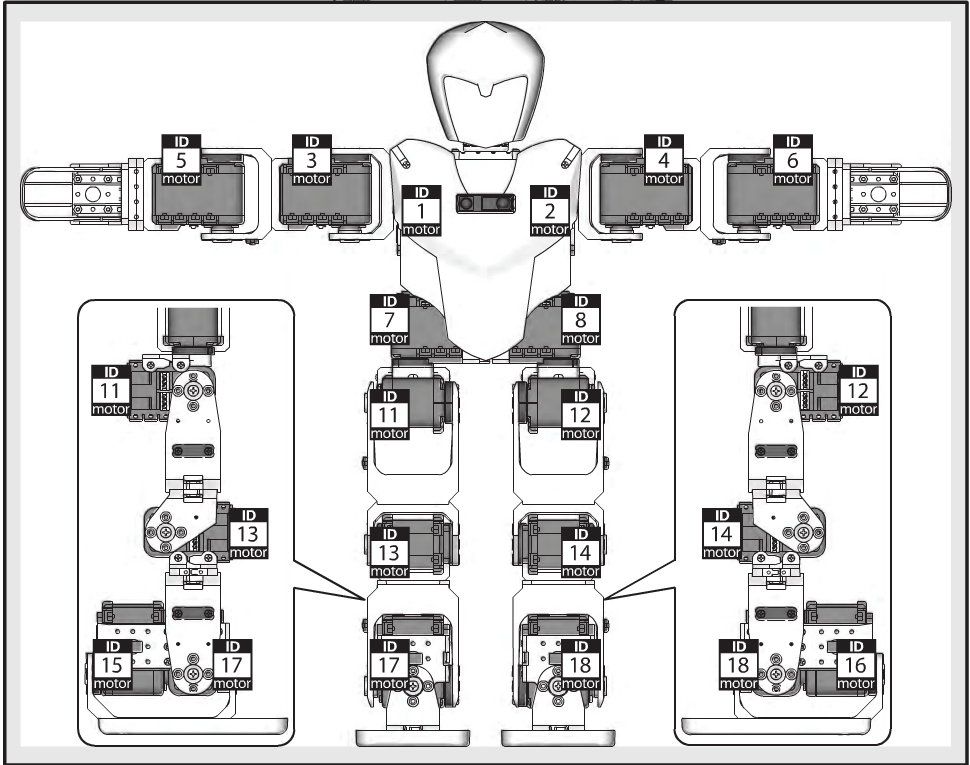
\includegraphics[scale=0.3]{imagenes/Robot.png}
\caption{Vista frontal del robot. Se puede apreciar la identificación ‘ID’ de cada motor Dynamixel Ax-12+. Nota: los motores 9 y 10 no se utilizan}
\label{fig:frontal}
\end{figure}

\begin{figure}[hbtp]
\centering
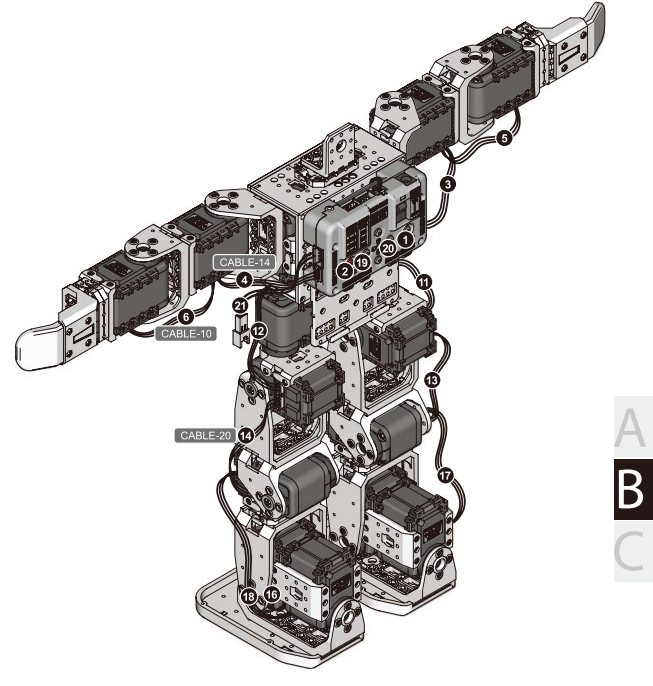
\includegraphics[scale=0.3]{imagenes/RobotTrasero.png}
\caption{Vista trasera del robot}
\label{fig:trasera1}
\end{figure}

El kit bioloid incluye una tarjeta controladora CM-510 la cual fue sustituida por la tarjeta controladora de software libre Arbotix. La utilización de la tarjeta Arbotix permite una mayor flexibilidad en el control de motores y la incorporación de una variedad de sensores no soportados por la tarjeta CM-510.
Además la tarjeta Arbotix posee mayor soporte y amplitud en la comunicación entre distintos dispositivos. 

En la figura ~\ref{fig:trasera2} se puede observar la estructura del robot con la Arbotix incorporada. En la parte interna del tronco del robot se sitúa el sensor Gyro.

\begin{figure}[hbtp]
\centering
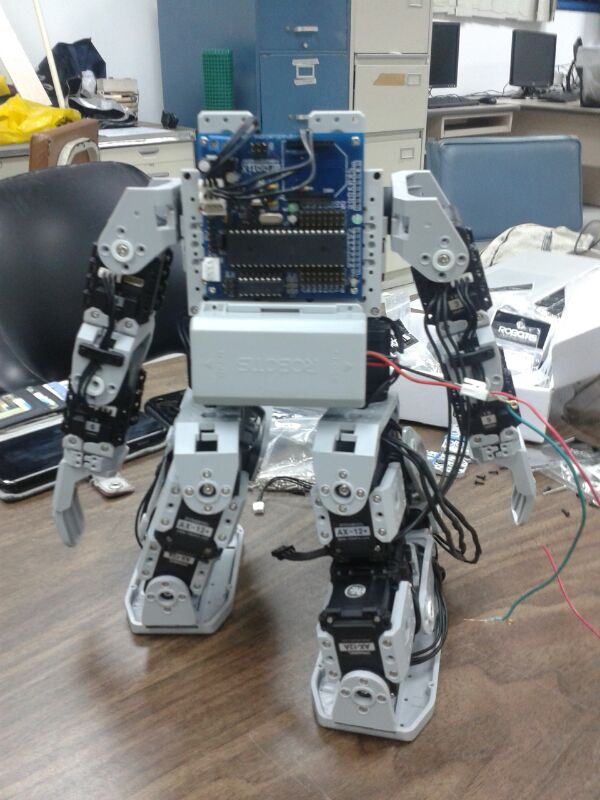
\includegraphics[scale=0.2]{imagenes/traseroDeJunny.jpg}
\caption{Vista trasera del robot con la Arbotix}
\label{fig:trasera2}
\end{figure}

\begin{figure}[hbtp]
\centering
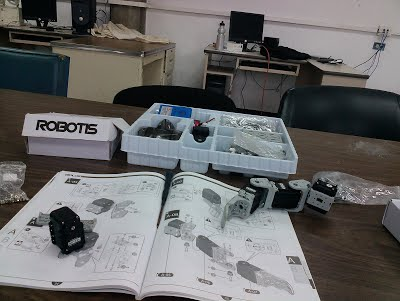
\includegraphics[scale=0.5]{imagenes/CIMG0225.jpg}
\caption{Manual de instrucciones y piezas del robot}
\end{figure}

Para el movimiento de la cámara se ha incorporado dos servomotores, uno para el movimiento horizontal y otro para el vertical. La conexión es pin a pin en los puertos especiales para ese tipo de motores (‘Hobby servos’) REF (ver figura ~\ref{fig:puertosHobby}). La cámara ha sido conectada a la Raspberry Pi en el puerto CSI (ver la figura ~\ref{fig:camACSI}). El resultado de estas tres piezas instaladas en el robot se puede apreciar en la figura ~\ref{fig:servosycam}.

\begin{figure}[hbtp]
\centering

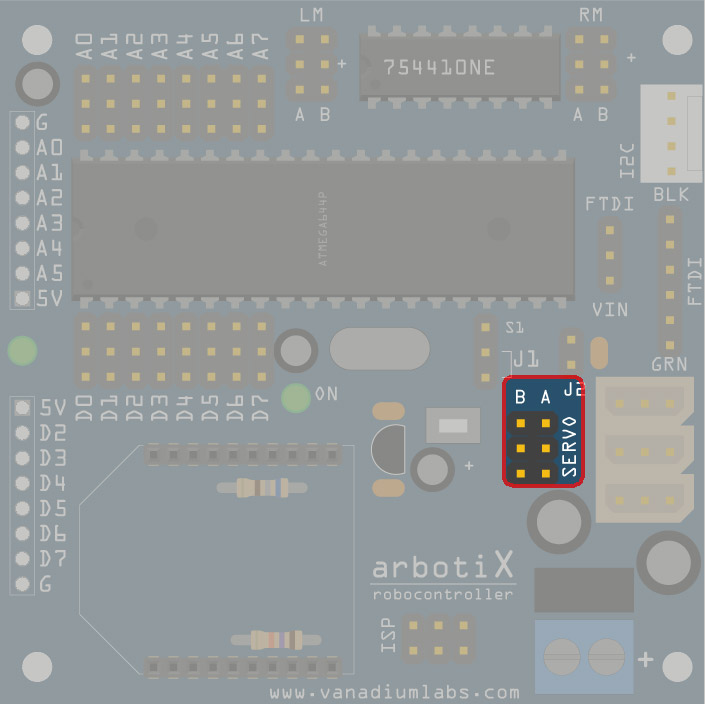
\includegraphics[scale=0.2]{imagenes/arbotix_hobby_servo.jpg}
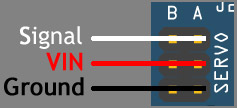
\includegraphics[scale=0.4]{imagenes/arbotix_hobbyservos_lines.jpg}
\caption{Ilustración de los puertos Hobby de la Arbotix}
\label{fig:puertosHobby}
\end{figure}

\begin{figure}[hbtp]
\centering
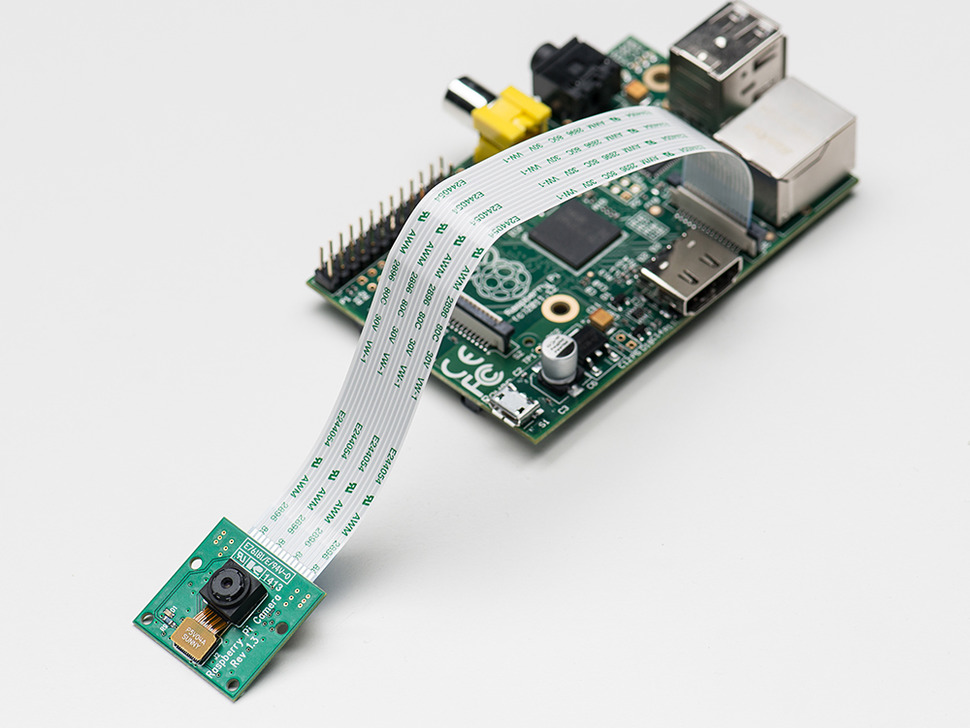
\includegraphics[scale=0.6]{imagenes/raspbCam.jpg}
\caption{C\'amara Raspberry Pi conectada al puerto CSI de la tarjeta}
\label{fig:camACSI}
\end{figure}
 
\begin{figure}[hbtp]
\centering
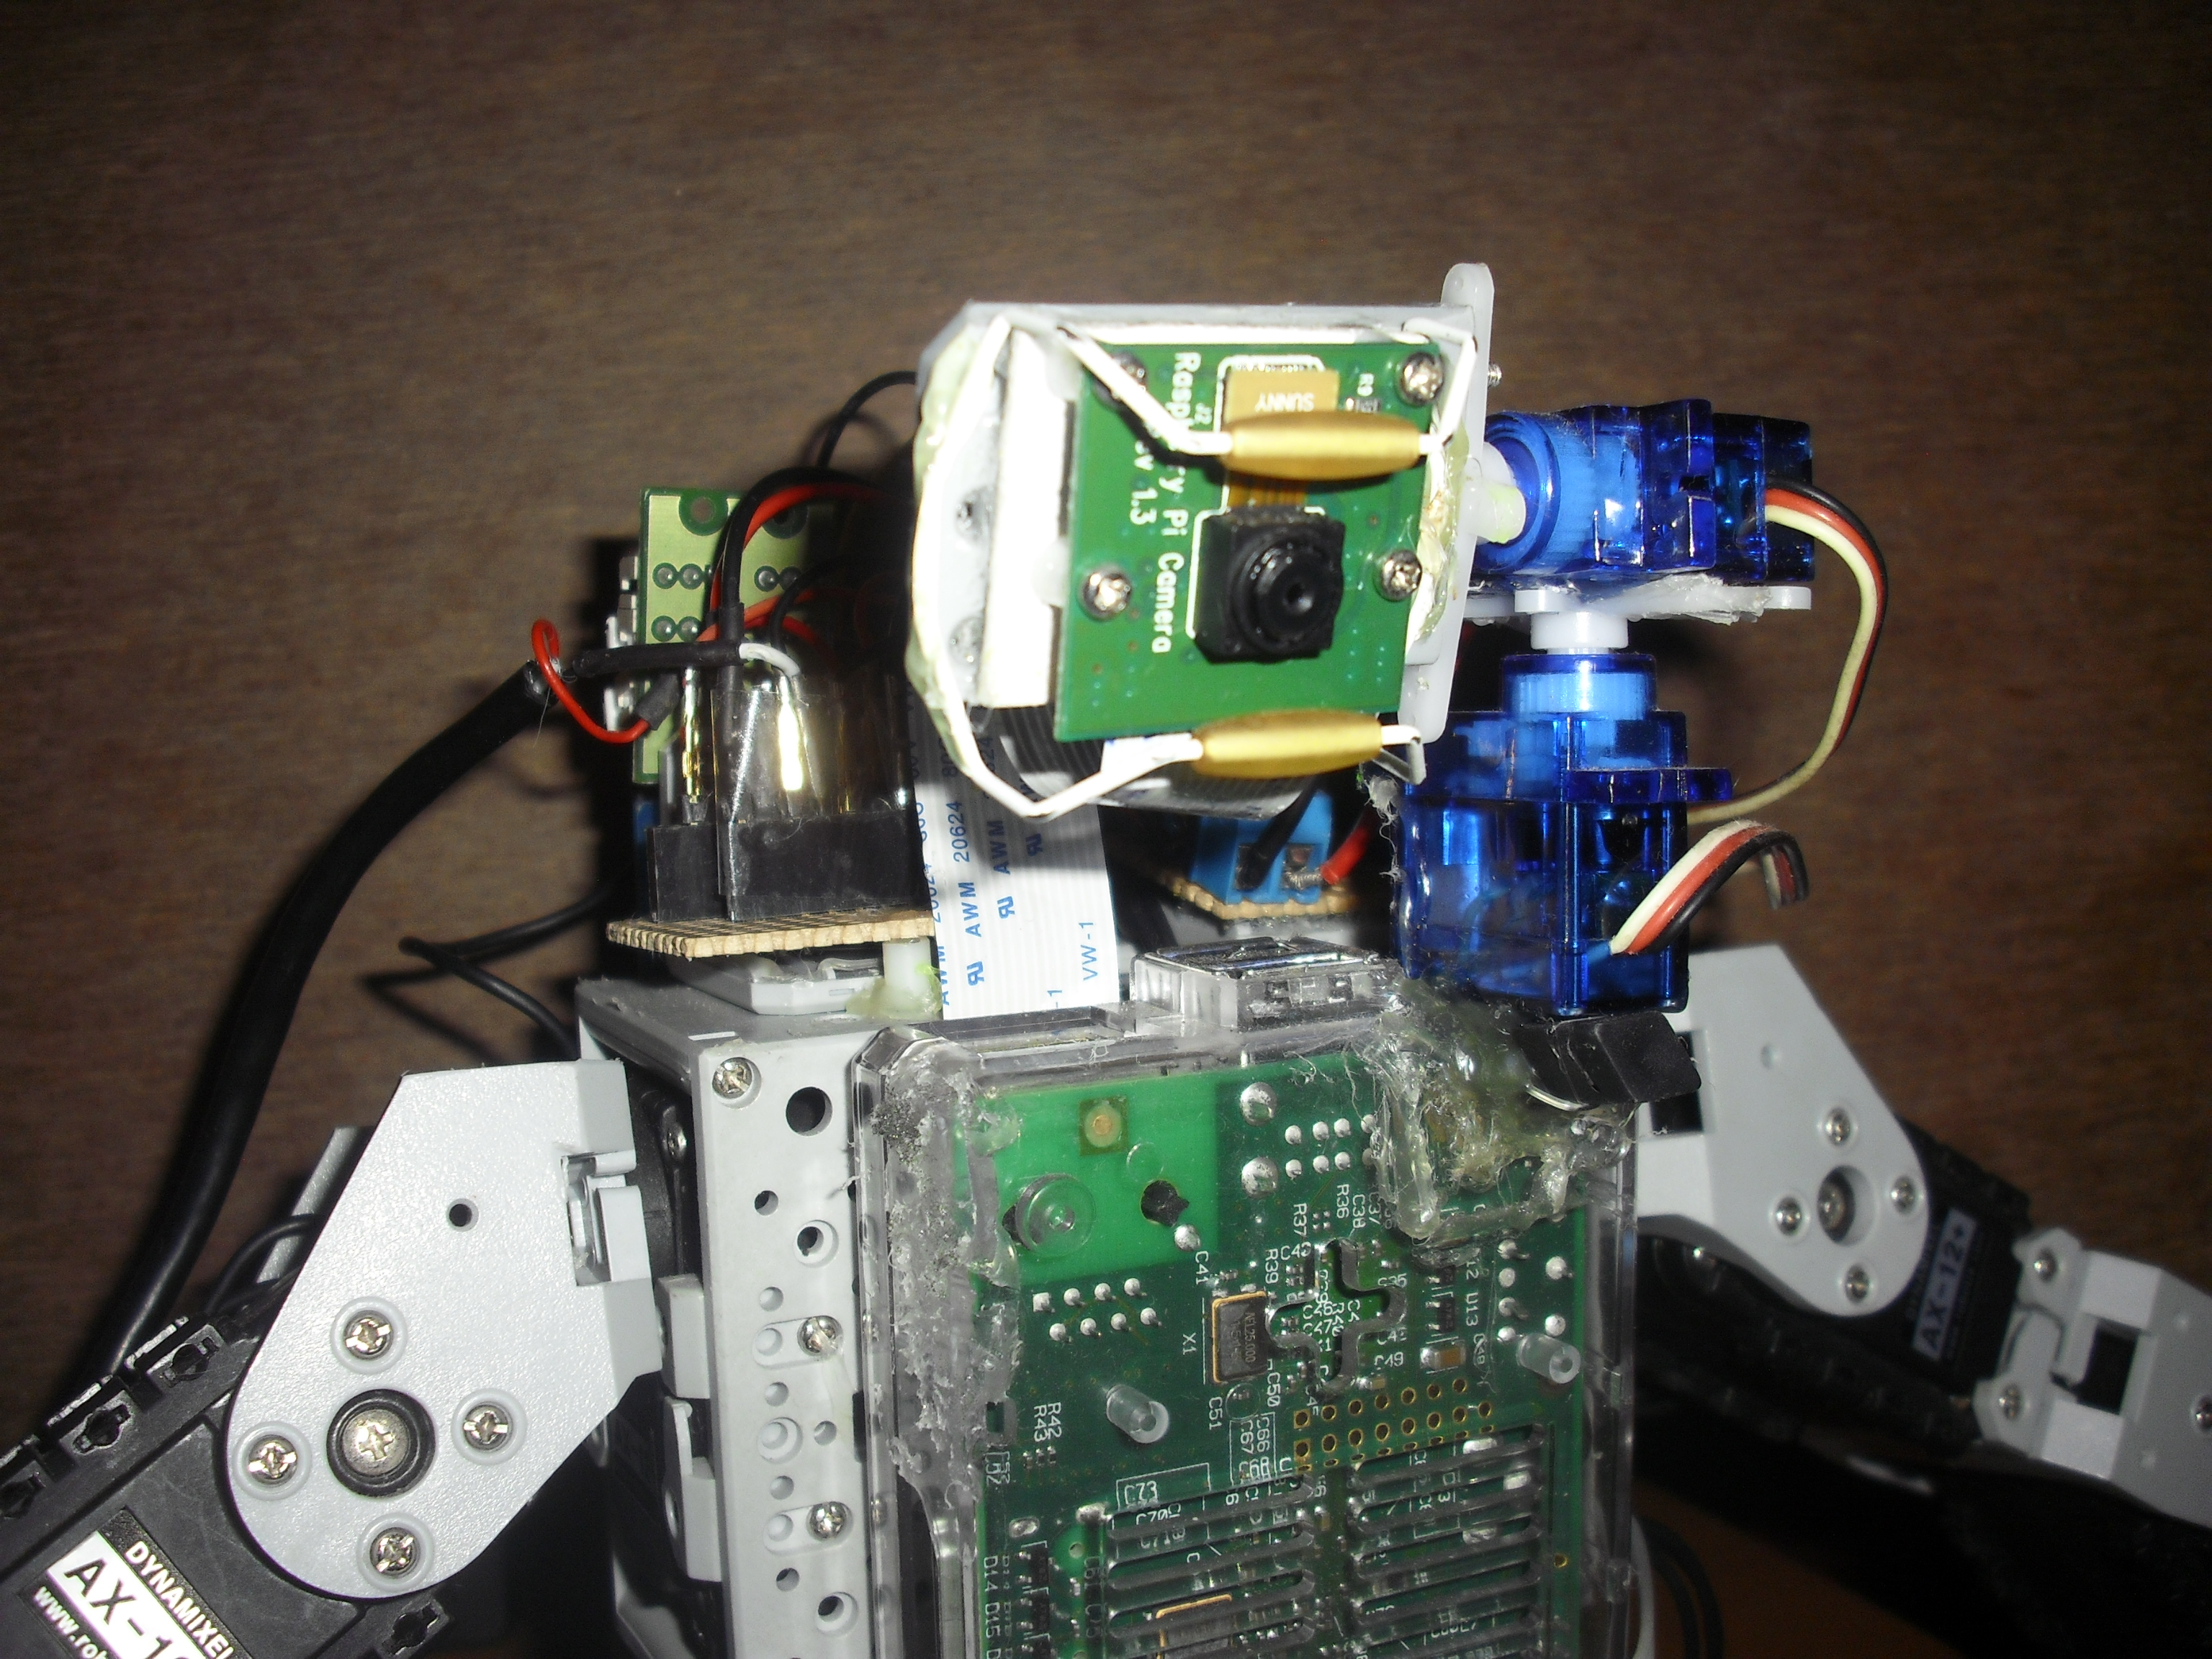
\includegraphics[scale=0.08]{imagenes/servosYcamara.JPG}
\caption{Vista delantera del robot con la cámara y servomotores instalados}
\label{fig:servosycam}
\end{figure}

Los motores Dynamixel se conectan a la controladora Arbotix por medio de los puertos bioloid de la tarjeta. La Arbotix s\'olo cuenta con tres puertos y el diseño del robot necesita cuatro series distintas 
una para cada extremidad por lo tanto cuatro puertos bioloid, se consideró la opción de unir dos extremidades pero ello implicaba limitaciones en el movimiento del robot por lo tanto se optó por agregar un expansor de puertos bioloid y así conectar cada extremidad en un puerto diferente. La forma en la que se ha conectado estos motores se ejemplifica en la figura ~\ref{fig:arbotixConectados}. 

\begin{figure}[hbtp]
\centering
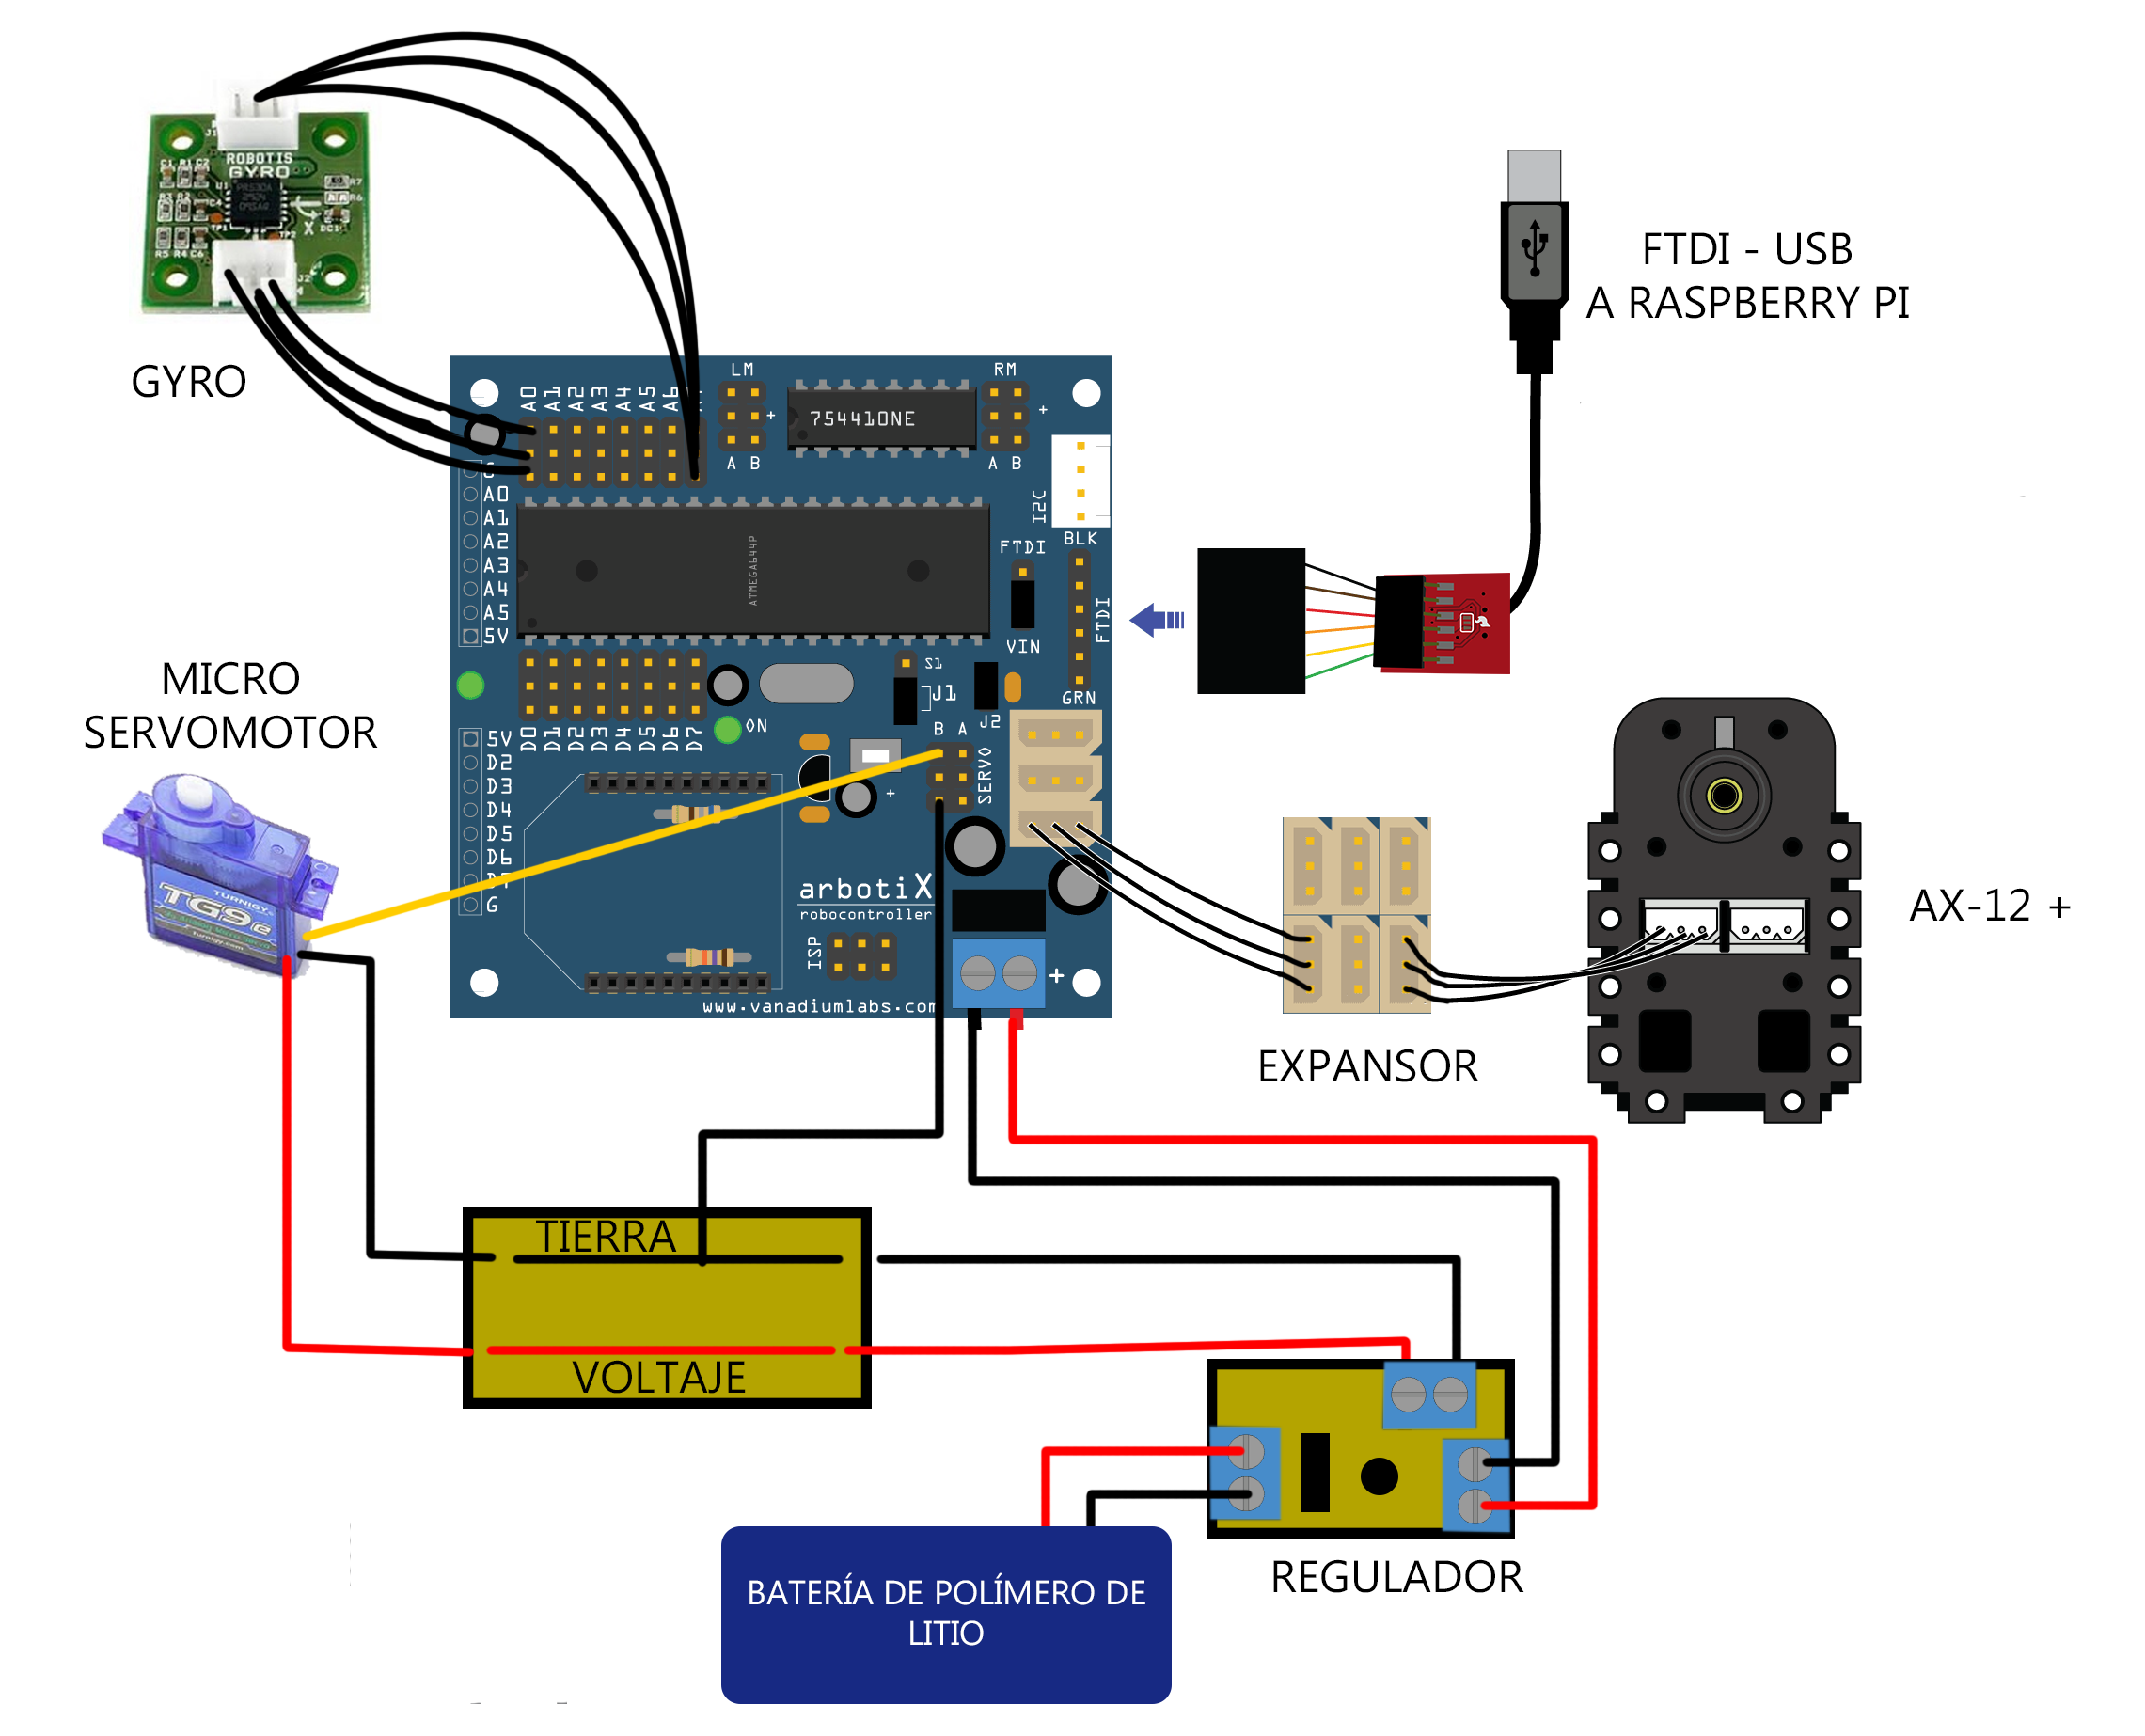
\includegraphics[scale=0.2]{imagenes/arbotix_servo.png}
\caption{Tarjeta controladora Arbotix y componentes conectados }
\label{fig:arbotixConectados}
\end{figure}

La comunicación de la tarjeta de Arbotix con la computadora, incluso con la Raspberry Pi, se realiza a través del puerto FTDI por medio un chip conectado como lo ilustra la figura ~\ref{fig:arbotixConectados}.

Como fuente de poder se utilizó una batería de polímero de litio de 11.1 V y 1 amp. Debido a que no todos los componentes poseen las mismas exigencias con respecto a voltaje y amperaje, se realizó un regulador (ver figura ~\ref{fig:circuito}) con  salida de 5 voltios para la tarjeta Raspberry Pi y los dos micro servomotores, con otra salida de 11.1 V para la tarjeta Arbotix que a su vez alimenta a los componentes conectados en ella (motores Dynamixel y Giroscopio). Si bien la tarjeta Arbotix posee un regulador interno de cinco voltios la opción de conectar todo a la salida de 5 V del regulador no era posible dado que los motores Dynamixel necesitan 11 voltios por lo tano se agregó la salida de 11.1 voltios.

\begin{figure}[hbtp]
\centering
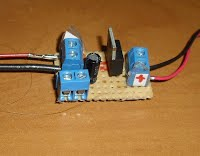
\includegraphics[scale=0.5]{imagenes/circuito.jpg}
\caption{Circuito con entrada de 11.1 V. Una salida de 5 V para los micro servomotores anal\'ogicos y tarjeta Raspberry Pi. Otra salida de 11 v para alimentar la controladora Arbotix.}
\label{fig:circuito}
\end{figure}

